\documentclass[10pt]{article}
\usepackage[utf8]{inputenc}
\usepackage[a4paper, margin=1cm, bottom=2cm]{geometry}
\usepackage{tabularx}
\usepackage{xcolor}
\usepackage{tikz}
\usepackage{graphicx}
\usepackage{times}
\usepackage{hyperref}
\usepackage{fancyhdr}
\usepackage{background}
\usepackage{fontawesome5}


\definecolor{dndred}{RGB}{120, 0, 0}

% Fundo estilo "papel envelhecido"
\backgroundsetup{
  scale=1,
  angle=0,
  opacity=1,
  contents={
\includegraphics[width=\paperwidth,height=\paperheight]{parchment.png}}
}

% Cores
\definecolor{icrpg}{RGB}{30,50,90}
\definecolor{caixacinza}{RGB}{230,225,210}

% Fonte medieval simulada
\newcommand{\medieval}[1]{\textcolor{dndred}{\textbf{\fontsize{12}{14}\selectfont\scshape #1}}}


% Campos editáveis
\newcommand{\smallfield}[1]{%
    \TextField[
        name=#1,
        width=1.2cm,
        height=0.4cm,
        bordercolor=black,
        backgroundcolor=white,
        charsize=14pt,
    ]{}%
}

\newcommand{\skillfield}[1]{%
    \TextField[
        name=#1,
        width=1.2cm,
        height=0.5cm,
        bordercolor=black,
        backgroundcolor=white,
        charsize=14pt,
    ]{}%
}

\newcommand{\editbox}[2][4.5cm]{%
    \TextField[
        name=#2,
        width=\linewidth,
        height=#1,
        bordercolor=black,
        backgroundcolor=white,
        charsize=9pt,
        multiline=true
    ]{}%
}

\newcommand{\smalltext}[1]{%
    \TextField[
        name=#1,
        width=1.8cm,
        height=0.25cm,
        bordercolor=black,
        backgroundcolor=white,
        charsize=11pt
    ]{}%
}

\newcommand{\mediumfield}[1]{%
    \TextField[
        name=#1,
        width=3.5cm,
        height=0.3cm,
        bordercolor=black,
        backgroundcolor=white,
        charsize=12pt
    ]{}%
}

\newcommand{\namefield}[1]{%
    \TextField[
        name=#1,
        width=10cm,
        height=0.9cm,
        bordercolor=black,
        backgroundcolor=white,
        charsize=20pt,
    ]{}%
}

% Início do documento
\begin{document}
\pagestyle{empty}
\color{black}

% Cabeçalho com nome e campos
\begin{center}
\vspace*{-1cm}
{\medieval{\fontsize{30}{32}\selectfont \namefield{charname}}} \\[10pt]
\small
\begin{tabularx}{0.9\textwidth}{XXX}
\medieval{World:} \mediumfield{world} &
\medieval{LF:} \mediumfield{lifeform} &
\medieval{Type:} \mediumfield{type} \\
\end{tabularx}
\end{center}

\vspace{5mm}
\hrule height 1pt
\vspace{8mm}

% Atributos, habilidades, imagem
\noindent
\begin{tabular}{@{}p{4.5cm}@{\hspace{6mm}}p{4.5cm}@{\hspace{6mm}}p{4.5cm}@{}}
% Atributos
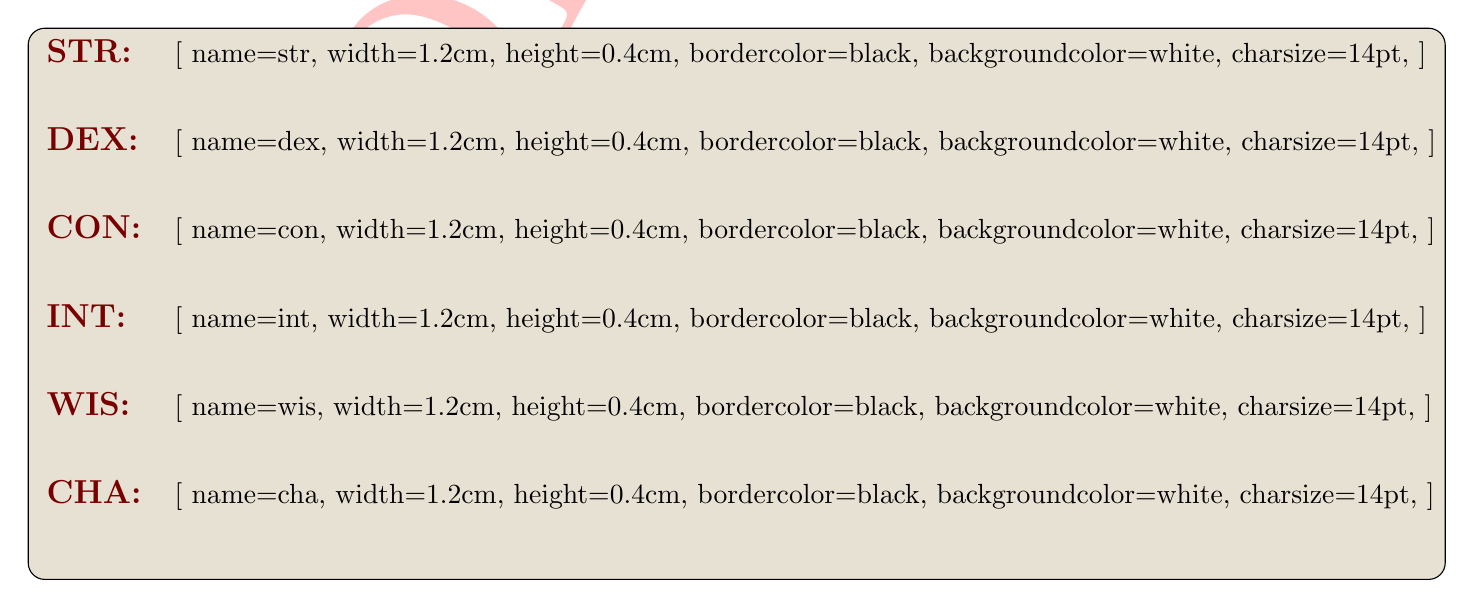
\begin{tikzpicture}
\node[fill=caixacinza, draw, minimum width=4.5cm, minimum height=7cm, rounded corners=6pt] {
\begin{tabular}{@{}ll@{}}
\vspace{0.5cm}
\medieval{STR:} & \smallfield{str} \\[2mm]
\vspace{0.5cm}
\medieval{DEX:} & \smallfield{dex} \\[2mm]
\vspace{0.5cm}
\medieval{CON:} & \smallfield{con} \\[2mm]
\vspace{0.5cm}
\medieval{INT:} & \smallfield{int} \\[2mm]
\vspace{0.5cm}
\medieval{WIS:} & \smallfield{wis} \\[2mm]
\vspace{0.5cm}
\medieval{CHA:} & \smallfield{cha} \\[2mm]
\end{tabular}
};
\end{tikzpicture}
&
% Skills
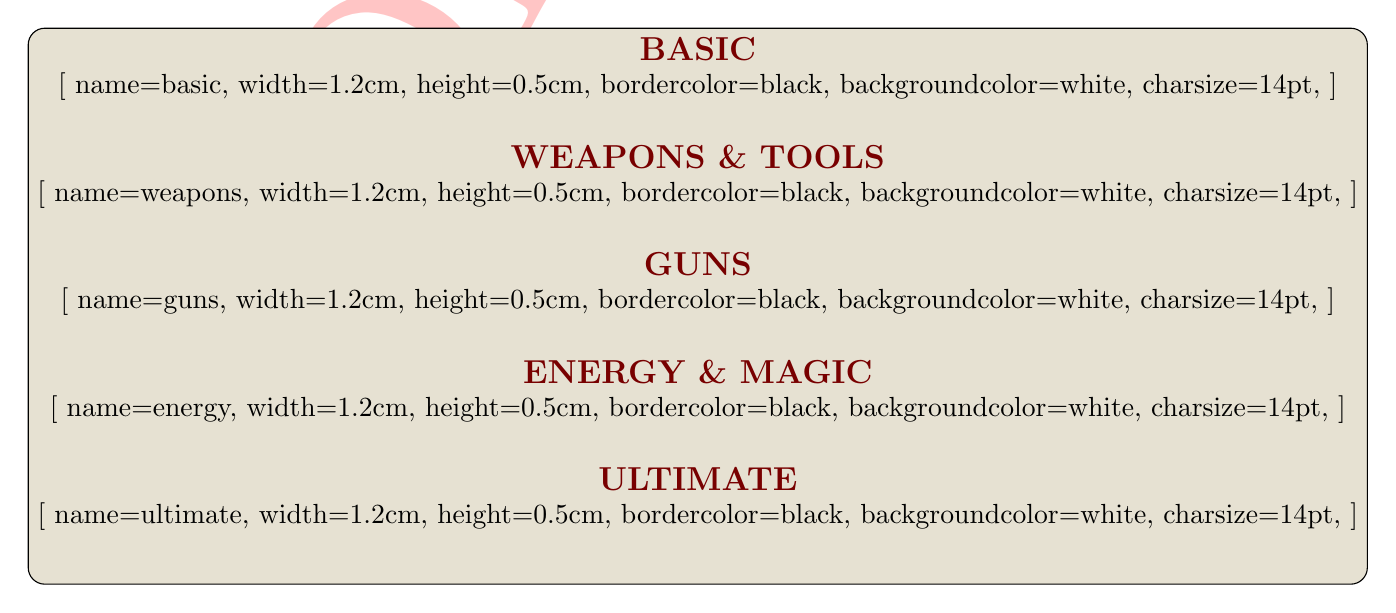
\begin{tikzpicture}
\node[fill=caixacinza, draw, minimum width=4.5cm, minimum height=7cm, rounded corners=6pt] {
\begin{tabular}{@{}c@{}}
\medieval{BASIC} \\ \skillfield{basic} \\[1mm] \\
\medieval{WEAPONS \& TOOLS} \\ \skillfield{weapons} \\[1mm] \\
\medieval{GUNS} \\ \skillfield{guns} \\[1mm] \\
\medieval{ENERGY \& MAGIC} \\ \skillfield{energy} \\[1mm] \\
\medieval{ULTIMATE} \\ \skillfield{ultimate} \\[1mm] \\
\end{tabular}

};
\end{tikzpicture}
&
% Imagem do personagem
\begin{tikzpicture}
\node[draw, minimum width=4.5cm, minimum height=7cm, rounded corners=6pt] {
\centering

\includegraphics[width=6cm,height=6cm]{Turner.jpg}
};
\end{tikzpicture}
\end{tabular}

\vspace{10mm}

% Linha com HP, DEF, etc.
\noindent
\begin{tikzpicture}
\node[fill=caixacinza, draw, minimum width=\textwidth, minimum height=1.5cm, rounded corners=6pt] {
\begin{tabular}{@{}llll@{}}
\medieval{HP:} \smalltext{hp} \hspace{0.5cm} & 
\medieval{DEFENSE:} \smalltext{defense} \hspace{0.5cm} &
\medieval{HERO COIN:} \smalltext{hero} \hspace{0.5cm} &
\medieval{DYING:} \smalltext{dying}
\end{tabular}
};
\end{tikzpicture}

\vspace{8mm}

% Loot e Abilities
\noindent
\begin{tabular}{@{}p{0.48\textwidth}p{0.48\textwidth}@{}}
\begin{tikzpicture}
\node[draw, fill=caixacinza, minimum width=\linewidth, minimum height=4cm, rounded corners=6pt] {
\begin{minipage}{\linewidth}
\medieval{LOOT}\\[2mm]
\editbox{loot}
\end{minipage}
};
\end{tikzpicture}
&
\begin{tikzpicture}
\node[draw, fill=caixacinza, minimum width=\linewidth, minimum height=4cm, rounded corners=6pt] {
\begin{minipage}{\linewidth}
\medieval{ABILITIES}\\[2mm]
\editbox{abilities}
\end{minipage}
};
\end{tikzpicture}
\end{tabular}

\vspace{8mm}

% Powers e Augments
\noindent
\begin{tabular}{@{}p{0.48\textwidth}p{0.48\textwidth}@{}}
\begin{tikzpicture}
\node[draw, fill=caixacinza, minimum width=\linewidth, minimum height=5.5cm, rounded corners=6pt] {
\begin{minipage}{\linewidth}
\medieval{POWERS}\\[2mm]
\editbox[5cm]{powers}
\end{minipage}
};
\end{tikzpicture}
&
\begin{tikzpicture}
\node[draw, fill=caixacinza, minimum width=\linewidth, minimum height=5.5cm, rounded corners=6pt] {
\begin{minipage}{\linewidth}
\medieval{AUGMENTS}\\[2mm]
\editbox[5cm]{augments}
\end{minipage}
};
\end{tikzpicture}
\end{tabular}

\newpage

% Página 2 - História
\begin{center}
    {\medieval{\fontsize{26}{30}\selectfont History}} \\[5mm]
\end{center}

\vspace{5mm}

\TextField[
    name=history,
    width=\textwidth,
    height=24cm,
    bordercolor=black,
    backgroundcolor=white,
    charsize=11pt,
    multiline=true
]{}

\vfill
\begin{center}
    {\small \textcolor{gray}{\faGithub\ \href{https://github.com/seuusuario}{https://github.com/Gabs-vhd/Ficha-ICRPG}}}
\end{center}

\end{document}
